\section{Proposed Method}
\label{sec:proposed_method}
\begin{figure*}[t]
    \centering
    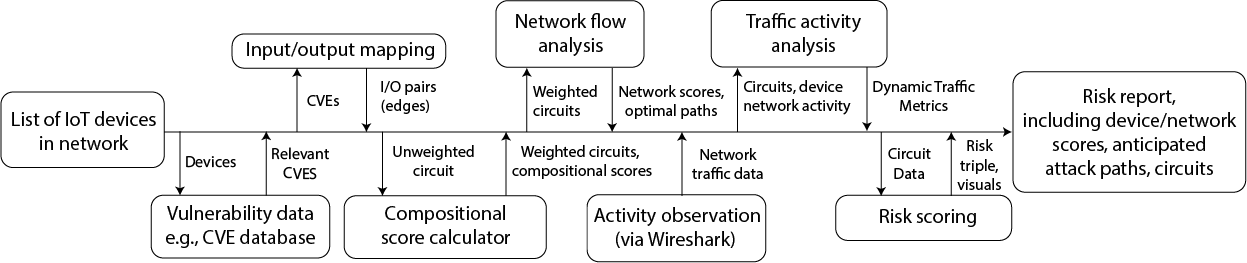
\includegraphics[width=\textwidth]{system_architecture.png}
    \caption{System architecture summary.}
    \label{fig:system_architecture}
\end{figure*}
Our proposal is a sequential computation of the triple $\langle R, E, I\rangle$---a method that utilizes preexisting knowledge about the devices in the network, topology of the network (determined by the relation between different vulnerabilities and potential network flow between devices), and dynamic device activity and network traffic information. This process is outlined in Figure \ref{fig:system_architecture}. At the practical level, the attack circuit model we are proposing considers each of these properties and can provide each of the desired metrics. An attack circuit is a type of flow network \cite{goldberg1989network}, wherein the flows can be used to evaluate level of risk, exploitability, and impact of a network, device, and vulnerability. In this section, we will discuss the nontrivial problem of constructing attack circuits using preexisting knowledge and inferences about IoT devices in the network. We will then explore how the network can then be used to compute \textit{compositional scores} on each of the vulnerabilities, which  provide an important baseline for understanding the initial risk, exploitability, and impact assessments of the network. Then, we'll examine the affect that dynamic network traffic behaviors have on the security of devices in the network and show how these \textit{dynamic metrics} can be combined with the compositional score for a more holistic look at the security of the IoT network. Finally, we'll propose the use of network flow algorithms that make use of the scores we've calculated for anticipating optimal attack paths, which give a final evaluation of the risk, exploitability, and impact measures of the network and its devices. A summary of the implemented system architecture is shown in Figure \ref{fig:system_architecture}.

% To produce a dense representation of possible attacks, the database of vulnerabilities is transformed into flow network graphs . Sources and sinks in the flow network correspond to attack sources and exploited system utilities (attacker targets) respectively. The paths from sources to sinks in the graph are then called \textit{attack circuits}.

\subsection{Circuit Construction}

The attack circuit is constructed in two stages, described in the following sections.

\subsubsection{Input/Output Extraction}
\label{subsubsec:input_output_extraction}

The attack circuits are modeled using text input (vulnerability descriptions) from a vulnerability database. For each item in the database, a corresponding \textit{input/output} pair is generated. The \textit{input} corresponds to the attack source and the \textit{output} corresponds to the attack target. The process is based on TF-IDF \cite{leskovec2014mining} and TextRank \cite{mihalcea2004textrank,PyTextRank} heuristics and is described next as a series of steps.

All text is primed by conversion to lowercase, removal of non-alphanumeric characters, tokenization, stemming \cite{porter1980algorithm,jones1997readings} and subsequent de-tokenization. TF-IDF is then used on the processed corpus to produce an ordering of tokens for each description. TextRank is used on the processed corpus to produce an ordered list of candidate phrases (with Part-Of-Speech (POS) tags) that may best represent the description. The ordered list is filtered to remove noun items (NN). For each item in the list, tokens pruned (limited to a maximum quantity of $3$) based on TF-IDF ordering. Stemming is then removed from tokens by matching them to the corresponding phrase. The result is stored as \textit{input}. This extraction process is then repeated using filtering to remove non-noun items and the result is stored as \textit{output}.

\subsubsection{Graph Composition}

After all of the \textit{input/output} pairs are created, we have the information we need to build the attack circuit structure. In our methodology, an attack circuit is a directed graph isomorphic to a flow network $C = (D,A,S,E)$ where $d \in D$ is a device, represented as a set of vertices that are the set of vulnerability database entries corresponding to $d$; $A$ is the set of attacker vertices; $S$ is the set of target (or sink, as we'll see later) vertices which represent the attack targets in the network; and $E$ is the set of labeled, directed edges. The attack circuit scheme suffices to provide a logical approach to determining which attack targets are at risk. We are more interested, however, in creating variants of the attack circuit that may give insight to the potential impact, exploitability, and overall risk an IoT network yields. To do this, we assign weights and capacities to each of the edges depending on the impact and expoitability scores associated with the respective vulnerability data. A device's impact, exploitability and base scores are then used to compute the attack vector corresponding to its vulnerability. This is used as a component of the device's risk score.

\subsection{Network Composition Analysis}

We're interested in taking a holistic look at devices when evaluating their levels of security and risk. We therefore use several different security metrics that may each be classified into one of two larger categories: compositional scoring and dynamic activity assessment, discussed in the next subsection. Compositional scoring may be performed by observing the device specification, associated vulnerability database information and their corresponding vulnerability scores, and attack circuit topology. Our work incorporates the first two items and designates the third for future work. These compositional scores are derived from the devices themselves and their role in the network composition, and can be calculated irrespective of ways the devices are being used over time. For our work, device's vulnerabilities are scored using the risk base, exploitability, and impact subscore method provided by the existing CVSS v3 standard which accompanies most CVEs. After computing the exploitability and impact subscores for each vulnerability, we can then calculate the compositional score ($c$) of each vulnerability, which is recursively computed using the impact weights and exploitability capacities of the edges of the graph. This is summarized in Equation \ref{eq:exploitability_score} and Equation \ref{eq:impact_score}, where $C_i$ is the set of attack circuit input vertices ($c_i$), where there exists an edge $(c_i,c)$, $C_o$ is the set of attack circuit output vertices ($c_o$), where there exists an edge $(c,c_o)$, and $v_d$ is a dampening constant. The impact and exploitability subscores of each vulnerability of a particular device are then assimilated and transformed (using sigmoidal activation) to determine the impact and exploitability subscores.

\begin{equation}
c_{Exploitability} \mathrel{+}= v_d\sum_{c_i}c_{i_{Exploitability}}
\label{eq:exploitability_score}
\end{equation}

\begin{equation}
c_{Impact} \mathrel{+}= v_d\sum_{c_o}c_{o_{Impact}}
\label{eq:impact_score}
\end{equation}

\subsection{Network Traffic Analysis}

We next examine the dynamic activity metric of a given device in the network. A large body of work is focused on abnormality detection and scoring in network traffic patterns \cite{acar2018peek,apthorpe2017spying,apthorpe2017smart}. A vast variety of metrics may be used for results that shed light onto particular aspects of IoT device and network security. Our work focuses on ascertaining a small number of these metrics from packet sniffing on the network of IoT devices over a period time. The data collected includes device traffic activity, packet content encryption, and the source/destination information of the packets.

To illustrate our use of device traffic activity information, consider the example shown in Figure \ref{fig:usage_over_time}. Devices that are online for the majority of the time (i.e. Google Home Mini, Roku Media Player, HP Printer, and Belkin WeMo) are assigned larger respective multipliers to their exploitability subscore, since their connection leaves them more open to attack by an adversary. The Amazon Echo Dot, in this case, does not have as significant a multiplier applied to its exploitability subscore, since it is not online as frequently.

\begin{figure}[t]
    \centering
    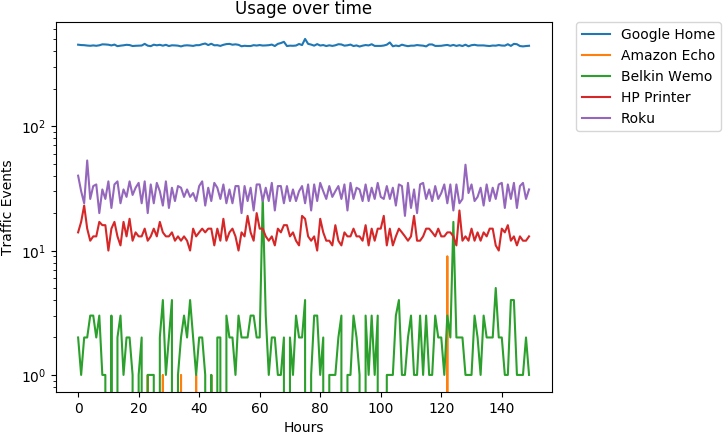
\includegraphics[width=0.5\textwidth]{usageJan14.png}
    \caption{An account of device traffic over a period of $12$ hours.}
    \label{fig:usage_over_time}
\end{figure}

Next, we analyze the percentage of the packets that are sent from and received by each device and their usage of secure encryption protocols. We also check whether any source or destination IP is listed in an IP blacklist database. The encryption metric is used as a multiplier for the exploitability subscore, and the blacklisted IP metric is used as a multiplier for the impact subscore. The calculated the compositional scores and dynamic activity metrics for a device can then be used to improve network analysis and security risk scoring.

\subsection{Network Flows and Attack Path Analysis}

To anticipate how an adversary might carry out an attack on the network and to score the network holistically, we apply a variety of \textit{Network Flow Problems} \cite{Ford-Fulkerson_algo} \cite{dantzig2003max} to the attack circuit for evaluating potential attack paths based on impact, exploitability, and risk. Sources and sinks in the flow network correspond to attack sources and attack targets, respectively.

\subsubsection{Impact Paths} 

An impact path is the route through the circuit that an attacker takes to maximize impact, defined by the circuit edge weights. We specify the attacker nodes as sources, and attacker targets as sinks. Equation \ref{eq:impact_path} illustrates the \textit{Maximum Flow Problem} method used--$f_{uv}$ is the flow between vertices $u$ and $v$, $a$ is an attacker vertex, $s$ is a sink (target) vertex. The sum of the impact path flows of an attack circuit (or the impact score of that circuit) are equivalent to the sum of the total impact of all \textit{easily} accessible attack targets, where the degree of accessibility is defined by the exploitability of the attack paths leading to it.

\begin{equation}
\begin{array}{ll@{}ll}
\text{maximize} & \displaystyle\sum\limits_{} f_{as} & \text{ subject to } \displaystyle\sum\limits_{j} f_{ji} = \displaystyle\sum\limits_{j} f_{ij}
\end{array}
\label{eq:impact_path}
\end{equation}

\subsubsection{Exploitability Paths} 

An exploitability path is a route from attacker to the attack target that is associated with a score  denoting the \textit{resistance} (intuitively, inverse exploitability) of that path. To determine the optimal exploitability paths in a circuit, we solve a \textit{Minimum Cost Flow Problem}, where the cost of an edge is its resistance, or the inverse of the exploitability of that edge (e.g. ($1-$Exploitability), if Exploitability $\in [0,1]$). We use the same sources and sinks as in Equation \ref{eq:impact_path} now with a cost $c_{ij}$ associated with edge $(i,j)$ and a required flow $r_{as}$ from attacker to sink (see Equation \ref{eq:exploitability_path}).

\begin{equation}
\begin{array}{ll@{}ll}
\text{minimize}  & \displaystyle\sum  c_{ij}f_{ij}
\text{ subject to } & \displaystyle\sum f_{as} = r_{as}
\end{array}
\label{eq:exploitability_path}
\end{equation}\\
After computing the optimal exploitability and impact paths, the paths themselves may serve as information for network operators. We may also sum over the exploitability paths in the network to determine an overall network exploitability score, which we then combine with the impact score to improve an overall network security risk score.

\subsubsection{Risk Flow Evaluation} 
Finally, we want to calculate high-risk paths and quantitatively apply these findings to our risk triple. A risk path is a route from attacker to target that is optimized for exploitability constraints, impact weights, and base compositional risk of the vertices. We combine the strategies used in exploitability path and impact path analysis here, solving a \textit{Minimum Cost Maximum Flow Problem} to identify likely paths through the IoT network that an adversary might use in an attack. In Equation \ref{eq:risk_mincost_path}, we outline the network flow problem used to calculate risk, with the usual $c_{ij}$ denoting cost of edge $(i,j)$, $a$ being an attacker vertex (source), and $s$ being a target vertex (sink):
\begin{equation}
\begin{array}{ll@{}ll}
\text{minimize } \displaystyle\sum c_{ij}f_{ij}
\text{ subject to: } \\
\ \ \ \ \text{maximize } \displaystyle\sum\limits_{} f_{as} \text{ subject to } \displaystyle\sum\limits_{j} f_{ji} = \displaystyle\sum\limits_{j} f_{ij}
\end{array}
\label{eq:risk_mincost_path}
\end{equation}
Computing risk paths allow us to calculate an improved risk triple for the network as well as the devices within. The triple $R = \langle R_{Conf}, R_{Integ}, R_{Avail} \rangle$ for a device is calculated using the CVSS v3 metrics for Confidentiality Impact, Integrity Impact, and Availability Impact associated with the CVEs of the device. Flow through each CVE is multiplied by the respective impact metric, and the result defines the risk triple $R$. The numerical values of the impact metrics may be found in table 8.4 of the CVSS v3 specification document\footnote{https://www.first.org/cvss/specification-document}.
% \begin{equation}
%     Base=\begin{cases}
%     0, & \text{Impact subscore $\leq$ 0}\\
%     \min(S_{\text{Impact}} + S_{\text{Exploitability}}, 10), & \text{Scope Unchanged}
    
%   \end{cases}\\
  
% \end{equation}
% \begin{equation}
% Impact=1-[(1-Impact_{\text{Conf}})(1-Impact_{\text{Integ}})(1-Impact_{\text{Avail}})]
% \end{equation}



%%%%%%%%%%%%%%%%%%%%